\documentclass{ieeeaccess}
\usepackage{cite}
\usepackage{amsmath,amssymb,amsfonts}
\usepackage{algorithmic}
\usepackage{graphicx}
\usepackage{textcomp}

\usepackage{tabularx}
\usepackage{balance}
\usepackage{multirow}%z
\usepackage{array} %Z
\usepackage{booktabs} %z
\usepackage[colorlinks=true, linkcolor=black, citecolor=black, urlcolor=black]{hyperref}

\def\BibTeX{{\rm B\kern-.05em{\sc i\kern-.025em b}\kern-.08em
    T\kern-.1667em\lower.7ex\hbox{E}\kern-.125emX}}

\begin{document}
\history{Date of publication xxxx 00, 0000, date of current version xxxx 00, 0000.}
\doi{10.1109/ACCESS.2023.0322000}

\title{Preparation of Papers for IEEE ACCESS}
\author{\uppercase{First A. Author}\authorrefmark{1}, \IEEEmembership{Fellow, IEEE},
\uppercase{Second B. Author}\authorrefmark{2}, and Third C. Author,
Jr.\authorrefmark{3},
\IEEEmembership{Member, IEEE}}

\address[1]{National Institute of Standards and
Technology, Boulder, CO 80305 USA (e-mail: author@boulder.nist.gov)}
\address[2]{Department of Physics, Colorado State University, Fort Collins,
CO 80523 USA (e-mail: author@lamar.colostate.edu)}
\address[3]{Electrical Engineering Department, University of Colorado, Boulder, CO
80309 USA}
\tfootnote{This paragraph of the first footnote will contain support
information, including sponsor and financial support acknowledgment. For
example, ``This work was supported in part by the U.S. Department of
Commerce under Grant BS123456.''}

\markboth
{Author \headeretal: Preparation of Papers for IEEE TRANSACTIONS and JOURNALS}
{Author \headeretal: Preparation of Papers for IEEE TRANSACTIONS and JOURNALS}

\corresp{Corresponding author: First A. Author (e-mail: author@ boulder.nist.gov).}


\begin{abstract}
This paper proposes a new method of tampered image detection by combining the CNN with a backbone of ResNet50 with ELA. Our method is designed for digital forensics, which is a very important domain for the detection and assessment of image modifications in many other domains, such as cybersecurity, journalism, and criminal investigations This procedure comprises image pre-processing to ascertain altered areas by comparing variations in compression levels to find compression artifacts using ELA. It serves as the foundation for reliable feature extraction: the ResNet50 model, pre-trained on ImageNet, has its basic layers frozen to preserve learned weights.
For customization with regard to binary classification, some custom layers are appended on top: global average pooling, batch normalization, dense layers with ReLU, and dropout regularization. The architecture here comes up with a generator-based approach so that large datasets can be handled with better memory consumption, enabling real-time data preprocessing during training of models.Our methodology is assured to optimize resource utilization and enhance generalization, which has been evidenced with extensive experiments. The obtained model offers high accuracy and robustness in detecting tampered images; thus, it presents a scalable solution for real-world forensic applications. This integration of ELA and CNN provides the backbone of fast and accurate analysis of digital evidence to help in better decision-making in sensitive situations.
\end{abstract}

\begin{keywords}
	Tampered Image Detection, Error Level Analysis (ELA), Convolutional Neural Network (CNN), ResNet50, Digital Forensics, Image Manipulation Detection, Cybersecurity, Journalism, Criminal Investigations, Feature Extraction, Binary Classification, Data Preprocessing, Dropout Regularization, Compression Artifacts, Real-time Analysis, Scalable Forensic Applications.
\end{keywords}

\titlepgskip=-21pt

\maketitle

\section{Introduction}
\label{sec:introduction}
\PARstart{I}{n} this digital era, where information is usually imparted through the means of digitization, a tampered image might start a wildfire of misinformation, controversies, and disasters in a lot of sectors. The more use of social media escalates the scale of it, which calls for this challenge to be taken seriously.The instances of tampered images being used for spreading fake news, malicing individuals or organizations, and manipulating public opinion have started becoming alarmingly common. A serious issue of this aspect, our research focuses on VeriForge, which is a model designed for the detection and exposure of image tampering using the powerful deep learning and Error Level Analysis~\cite{gupta2022detection}. This innovative approach is targeted at offering an effective solution in finding discrepancies in digital images and building trust in visual content. But accessibility to sophisticated image editing software has put the art of doctoring images within everybody's reach, irrespective of any kind of technical expertise. For that reason, it has become an increasingly demanding task to differentiate between original and tampered images by commoners, but also by professionals in vital fields like law and order or journalism. But available techniques of image tampering detection, though at one's fingertips, are not short-circuited by numerous limitations. Most of the known methods are outdated, slowing down, and cannot find a complex type of manipulation. Nowadays, there is a serious demand to create modern and effective methods which could cope with complications arising in image forgery techniques~\cite{kaur2019weak}.

VeriForge fills this gap by using the synergy of traditional forensic methods and deep learning. ELA, for example, is a well-established method in forensics: it underlines inconsistencies between image compression levels, hence highlighting the image anomalies caused by editing~\cite{singh2021image}. VeriForge couples ELA with deep learning to extract meaningful features from these discrepancies in a way that has allowed the attainment of high accuracy enabled by advanced neural network architecture. It allows VeriForge to find the tampered images with quite an intelligent attack.

For the training and verification of VeriForge, we utilize CASIA V2, a database of well-labeled images in their original and forged aspects. In this database, tampering is performed manually with several image editing tools; thus, it is one of the good sources for training a model to detect different types of tampering~\cite{7412439}. This is also ensured by the great variety of images in the dataset, thus the model generalizes well to unseen data, avoiding overfitting and improving its application in real-world scenarios.

The VGG-16 architecture was adopted for the first version of VeriForge. Although a promising result could be achieved in a preliminary way, we obtained only mediocre performance, given that after some point the model converged, resulting in an inability to increase its accuracy. Then, in order to capture the intricate image features, residual learning with the much deeper convolutional neural network architecture, ResNet50~\cite{simonyan2015deepconvolutionalnetworkslargescale}, was chosen. This switch to ResNet50 allowed VeriForge to capture more complicated patterns of tampered images, thereby increasing its detection capability by a big margin.


The general objective of the work is to protect the integrity of digital content by offering a reliable, scalable, and efficient tool for image forgery detection. In this regard, VeriForge uses advanced techniques such as convolutional neural networks (CNNs) ~\cite{thepade2021image}, transfer learning~\cite{han2020scene} , and state-of-the-art architectures like ResNet50~\cite{he2016deep} . Put together, these technologies ensure that VeriForge will find tampered images and continually improve by keeping pace with the changing world of image manipulation.

In a nutshell, VeriForge is a leap into the future of image tampering detection: it merges classical forensic techniques-such as ELA-with the latest powers of deep learning for an emerging need to have reliable tools safeguarding digital content in this world where visual communication is well on its way to dominating other forms.




\section{PROPOSED METHOD}

In this paper, we demonstrate that combining ELA with CNN model while freezing the base layers and adding custom layers to the base model which will provide a significant increase in the robustness of the final model and significantly improve performance of the classification task to detect images, which are tampered. We explore this idea in the context of digital forensics, where the goals are to analyze the images and detect suspicious activity in the field of crime, journalism etc. Since digital forensics helps uncover activities and patterns, determine the root causes of incidents, and establish a chain of evidence admissible in court, it becomes essential to identify, recover, analyze and present digital evidence from electronic devices and digital storage. Additionally, an ELA based model helps in identifying the difference in various layers of the images to help us uncover the underlying changes made to the image that is suspected to be tampered with. The model allows us to help various fields where criminal investigations, legal disputes and cybersecurity incidents occur and images need to be analyzed quicky to help user make quick informed decisions. The following sections outline the details of each step in the process.

\subsection{Initialization}

The initialization of the framework is preprocessing the images based on the number of images available in the dataset, it corresponds to the total number of images which are categorized in two classes specifically: 1) Authentic and 2) Tampered. The classes with their labels are split initially to ensure we have a sizeable amount of image to work with, we ensure that the classes are not biased and are equally balanced to provide a robust model and reduce overfitting. The classes are initialized with ones and zeros, zero if the image is authentic and one if the image has been tampered. For images to get preprocessed, we need to handle a chuck of images at a time, which will require us to take images in batches to preprocess and analyze further. 

After reshaping the images according to our input shape which will reduce the size of the image so that our next function would work effectively. Creating batches to handle memory overflow and preprocessing image before feeding them to the ELA function ensures that the system doesn’t require a lot of resources and is more optimized to create a more robust model.

Further, we take each resized image and input it to our ELA function, this step is iterated over multiple images to get robust images with reduced quality  to take forward for our ELA function.

\begin{figure*}
	\centering
	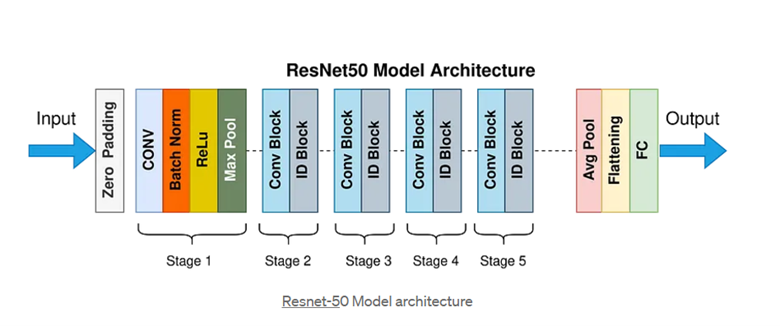
\includegraphics[width=\linewidth]{Base_Model.png}
	\caption{ Architecture of the base model}
	\label{base-model}
\end{figure*} 

\subsection{ELA Process with Generators}
For each image in our ELA function, we generate a buffer to save the original image to a temporary in-memory file with reduced quality, which helps us in reducing the overall memory utilization of the system. We load the compressed image from the buffer and calculate the difference between the original image and the one which was compressed to get the Pillow image object, this is a technique used in image forensics to detect tampering or inconsistencies in an image. We enhance the brightness of the image according to the extrema we get in the pillow image object. 

This returns us the ELA image which is a new image that emphasizes regions with differing compression levels, useful for detecting tampering or manipulation. This image will highlight differences due to compression artifacts. To feed the image forward to the model for training, it requires the image to be converted to an array for numerical processing and is normalized making the data compatible with many machine learning models. We close the image further to free up resources and it is a good practice to avoid file locks or memory leaks, especially when processing multiple images in a loop. For the model to handle such large number of images at once would require a lot of resources, to tackle this issue we provide generators to the model.

These generators help in handle image preprocessing and feeding batches of data to the model during training. They are often used in deep learning workflows when the model requires to load images in batches and apply transformations or augmentation. Instead of loading all images into memory at once, generators load and process batches on-the-fly, reducing memory consumption. Generators often include on-the-fly preprocessing, which enhances the dataset and helps the model generalize better, increasing its robustness and generalizability for better performance.
We also try to visualize the batch of images after the ELA function to ensure that the 	shape of the generator and preprocessed images are according to the requirements.

\subsection{Resnet50 Model Architecture with Training Evolution }
In this study, we employ a Resnet50 model to classify the images into two categories (Authentic and Tampered), we use a transfer learning approach based on the ResNet50 architecture, pre-trained on ImageNet to solve our classification problem. This method capitalizes on the robust feature extraction capabilities of ResNet50, significantly reducing training time and computational resources while improving model accuracy. The model was customized to adapt the pre-trained base for the task by introducing additional trainable (Custom) layers specifically designed for binary classification.Figure ~\ref{base-model}: shows the architecture of the base model we have used featuring Resnet50 in a five-stage design to represent the overall function of the layers

The base of our architecture is the ResNet50 model, known for its depth and efficient handling of the vanishing gradient problem through residual connections. The model was loaded without the top layers, removing the full-connected top layers helped us retained only the convolutional layers which are responsible for extracting hierarchical features from the input images. The input shape was fixed to match the requirement of the model while ensuring compatibility with pre-trained weights. The freezing of all layers in the base model during training aimed at preserving the learned weights and keeping the feature extraction capability unaltered by the new task-specific data. To this binary classification problem, we attached five different types of custom layers to the base pre-trained model in an attempt to make it adapt. First, there is a global average pooling layer that reduces the high-dimensional feature maps output by ResNet50 into a single vector for each feature map, reducing the number of trainable parameters and hence improving generalization. Unlike the traditional Flatten layer, this preserves spatial information and improves model performance when using ResNet-based architectures. Further, we added batch normalization to normalize the activations from the pooling layer, reducing internal covariate shift and accelerating convergence. 

Once we are done with that, we added a series of two dense layers. The first layer consists of 512 neurons providing substantial capacity to capture complex patterns. The second contains 256 neurons for further refinement of feature extraction. Both are activated by the ReLU activation function, which introduces non-linearity in deep networks and provides output zero for negative inputs, creating sparsity in the activations that could further be helpful in efficient computations with a reduction in overfitting. While being computationally less expensive than sigmoid or tanh function. The custom layers then involved a dropout regularization technique which was employed after each dense layer to with a rate of 0.75 after the first dense layer to impose strong regularization and rate of 0.5 was applied after the second dense layer for moderate regularization. This helped in preventing overfitting of the model during training. After dropout regularization, there was a single neuron in the output layer with sigmoid activation to predict the probability of the positive class, which is suitable for binary classification tasks.

It achieves a very good trade-off among accuracy, training efficiency, and robustness, making it pretty effective in real-world applications. This model was trained for more than 100 epochs with a step size of about 145 while capturing essential evaluation metrics such as accuracy, the f1 score, and validation accuracy. This will make sure we minimize the gap between the training and validation accuracy of the model, which will be robust and very effective in real-world applications.



\section{Results and Analysis}
	\begin{table}[h!]
\subsection{Datasets}
	The CASIA V2 dataset, created by the Institute of Automation at the Chinese Academy of Sciences, CASIA, is one of the more general resources for research in the area of image forgery detection. Designed to support studies on image tampering, it includes manipulative techniques such as splicing, copy-move forgery, and other methods.The Table~\ref{casiav2overview} outlines the details of the dataset and gives us an overview of what the dataset contains. The dataset is a very diverse collection of 12,614 images of roughly equal amounts of authentic and tampered examples from various categories such as nature, animals, objects, and urban settings. Such diversity will enable models trained with CASIA V2 to generalize rather well across different scenarios. There are also ground truth masks provided for every tampered image in the dataset, highlighting manipulated regions and thus making the dataset indispensable for supervised learning tasks and performance evaluation.
	
	The resolution of the images also varies to reflect real-world conditions, as images naturally come from different devices and sources.CASIA V2 has a variety of applications, including training and validation of image forgery detection models, testing of pre-processing techniques such as Error Level Analysis, and benchmarking deep learning architectures like CNNs for forgery classification. Features such as these make it invaluable in the field of digital forensics and research on image authenticity.
	

	\centering
	\setlength{\tabcolsep}{3pt}
	\vspace{3mm}
	\begin{tabular}{|p{75pt}|p{150pt}|p{115pt}|}
		\hline
		\textbf{Feature}            & \textbf{Description}                                                                 \\ \hline
		\textbf{Dataset Name}       & CASIA TIDE v2.0                                                                      \\ \hline
		\textbf{Purpose}            & Designed for research and development in image forgery detection                     \\ \hline
		\textbf{Released By}        & Chinese Academy of Sciences Institute of Automation (CASIA)                          \\ \hline
		\textbf{Image Type}         & Digital images, both authentic and tampered                                          \\ \hline
		\textbf{Number of Images}   & 12,614 images (7,491 authentic and 5,123 tampered)                                   \\ \hline
		\textbf{Forgery Techniques} & Splicing, copy-move, and other common image tampering techniques                      \\ \hline
		\textbf{Resolution}         & Varies (typically medium resolution)                                                 \\ \hline
		\textbf{File Format}        & JPEG (for compressed images)                                                         \\ \hline
		\textbf{Dataset Structure}  & Contains two folders: one for authentic images and one for tampered images           \\ \hline
		\textbf{Applications}       & Used for image forgery detection, digital forensics, and tampered image localization research \\ \hline
		\textbf{Public Availability} & Available for academic and non-commercial use upon request from CASIA               \\ \hline
	\end{tabular}
	\caption{Overview of the CASIA TIDE v2.0 Dataset}
	\label{casiav2overview}
\end{table}

\section{Conclusion}
This study is essential in maintaining integrity is crucial in fields like Law enforcement, Cyber security, and Legal investigations. In this project, we aimed to design a robust system capable of determining whether an image is tampered with. The research compares the performance of two widely known CNN models, VGG16 and ResNet50, with traditional preprocessing methods like ELA and data augmentation. The project concludes with viable results that taking colour inconsistencies and compression differences significantly improves model capability compared to conventional grayscale-based ELA methods.The system can be integrated into social media to moderate content in real-time, flagging misleading images and advancing platform integrity. In journalism, it makes sure that media is authentic by verifying images before publication; this helps in debunking fake news and fosters ethical reporting as a way of maintaining the public's trust in digital journalism.Although promising performance may be seen in the CASIA v2 dataset, it does not generalize upon exposure to other datasets or real-world scenarios. This needs to be handled in future work by enrichment of the dataset with diversity and updates for further strengthening the resistance and longevity of the model. Moreover, interpreting it with Explainable AI by using Grad-CAM will illustrate the regions of interest influential in the model's choices for transparent decisions and gaining the trust of the users.
The dataset and code for further research are available \href{https://www.kaggle.com/datasets/divg07/casia-20-image-tampering-detection-dataset/data}{[here]} and \href{https://github.com/ayaz168/veriforge}{[repository link]}.




\section*{Acknowledgment}
The preferred spelling of the word ``acknowledgment'' in American English is
without an ``e'' after the ``g.'' Use the singular heading even if you have
many acknowledgments. Avoid expressions such as ``One of us (S.B.A.) would
like to thank $\ldots$ .'' Instead, write ``F. A. Author thanks $\ldots$ .'' In most
cases, sponsor and financial support acknowledgments are placed in the
unnumbered footnote on the first page, not here.

\balance
\bibliographystyle{IEEEtran}
\bibliography{sn-bibliography.bib}

%\begin{thebibliography}{00}
%
%\bibitem{b1} G. O. Young, ``Synthetic structure of industrial plastics,'' in \emph{Plastics,} 2\textsuperscript{nd} ed., vol. 3, J. Peters, Ed. New York, NY, USA: McGraw-Hill, 1964, pp. 15--64.
%
%\bibitem{b2} W.-K. Chen, \emph{Linear Networks and Systems.} Belmont, CA, USA: Wadsworth, 1993, pp. 123--135.
%
%\bibitem{b3} J. U. Duncombe, ``Infrared navigation---Part I: An assessment of feasibility,'' \emph{IEEE Trans. Electron Devices}, vol. ED-11, no. 1, pp. 34--39, Jan. 1959, 10.1109/TED.2016.2628402.
%
%\bibitem{b4} E. P. Wigner, ``Theory of traveling-wave optical laser,'' \emph{Phys. Rev}., vol. 134, pp. A635--A646, Dec. 1965.
%
%\bibitem{b5} E. H. Miller, ``A note on reflector arrays,'' \emph{IEEE Trans. Antennas Propagat}., to be published.
%
%\bibitem{b6} E. E. Reber, R. L. Michell, and C. J. Carter, ``Oxygen absorption in the earth's atmosphere,'' Aerospace Corp., Los Angeles, CA, USA, Tech. Rep. TR-0200 (4230-46)-3, Nov. 1988.
%
%\bibitem{b7} J. H. Davis and J. R. Cogdell, ``Calibration program for the 16-foot antenna,'' Elect. Eng. Res. Lab., Univ. Texas, Austin, TX, USA, Tech. Memo. NGL-006-69-3, Nov. 15, 1987.
%
%\bibitem{b8} \emph{Transmission Systems for Communications}, 3\textsuperscript{rd} ed., Western Electric Co., Winston-Salem, NC, USA, 1985, pp. 44--60.
%
%\bibitem{b9} \emph{Motorola Semiconductor Data Manual}, Motorola Semiconductor Products Inc., Phoenix, AZ, USA, 1989.
%
%\bibitem{b10} G. O. Young, ``Synthetic structure of industrial
%plastics,'' in Plastics, vol. 3, Polymers of Hexadromicon, J. Peters,
%Ed., 2\textsuperscript{nd} ed. New York, NY, USA: McGraw-Hill, 1964, pp. 15-64.
%[Online]. Available:
%\underline{http://www.bookref.com}.
%
%\bibitem{b11} \emph{The Founders' Constitution}, Philip B. Kurland
%and Ralph Lerner, eds., Chicago, IL, USA: Univ. Chicago Press, 1987.
%[Online]. Available: \underline{http://press-pubs.uchicago.edu/founders/}
%
%\bibitem{b12} The Terahertz Wave eBook. ZOmega Terahertz Corp., 2014.
%[Online]. Available:
%\underline{http://dl.z-thz.com/eBook/zomegaebookpdf\_1206\_sr.pdf}. Accessed on: May 19, 2014.
%
%\bibitem{b13} Philip B. Kurland and Ralph Lerner, eds., \emph{The
%Founders' Constitution.} Chicago, IL, USA: Univ. of Chicago Press,
%1987, Accessed on: Feb. 28, 2010, [Online] Available:
%\underline{http://press-pubs.uchicago.edu/founders/}
%
%\bibitem{b14} J. S. Turner, ``New directions in communications,'' \emph{IEEE J. Sel. Areas Commun}., vol. 13, no. 1, pp. 11-23, Jan. 1995.
%
%\bibitem{b15} W. P. Risk, G. S. Kino, and H. J. Shaw, ``Fiber-optic frequency shifter using a surface acoustic wave incident at an oblique angle,'' \emph{Opt. Lett.}, vol. 11, no. 2, pp. 115--117, Feb. 1986.
%
%\bibitem{b16} P. Kopyt \emph{et al., ``}Electric properties of graphene-based conductive layers from DC up to terahertz range,'' \emph{IEEE THz Sci. Technol.,} to be published. DOI: 10.1109/TTHZ.2016.2544142.
%
%\bibitem{b17} PROCESS Corporation, Boston, MA, USA. Intranets:
%Internet technologies deployed behind the firewall for corporate
%productivity. Presented at INET96 Annual Meeting. [Online].
%Available: \underline{http://home.process.com/Intranets/wp2.htp}
%
%\bibitem{b18} R. J. Hijmans and J. van Etten, ``Raster: Geographic analysis and modeling with raster data,'' R Package Version 2.0-12, Jan. 12, 2012. [Online]. Available: \underline {http://CRAN.R-project.org/package=raster}
%
%\bibitem{b19} Teralyzer. Lytera UG, Kirchhain, Germany [Online].
%Available:
%\underline{http://www.lytera.de/Terahertz\_THz\_Spectroscopy.php?id=home}, Accessed on: Jun. 5, 2014.
%
%\bibitem{b20} U.S. House. 102\textsuperscript{nd} Congress, 1\textsuperscript{st} Session. (1991, Jan. 11). \emph{H. Con. Res. 1, Sense of the Congress on Approval of}  \emph{Military Action}. [Online]. Available: LEXIS Library: GENFED File: BILLS
%
%\bibitem{b21} Musical toothbrush with mirror, by L.M.R. Brooks. (1992, May 19). Patent D 326 189 [Online]. Available: NEXIS Library: LEXPAT File: DES
%
%\bibitem{b22} D. B. Payne and J. R. Stern, ``Wavelength-switched pas- sively coupled single-mode optical network,'' in \emph{Proc. IOOC-ECOC,} Boston, MA, USA, 1985, pp. 585--590.
%
%\bibitem{b23} D. Ebehard and E. Voges, ``Digital single sideband detection for interferometric sensors,'' presented at the \emph{2\textsuperscript{nd} Int. Conf. Optical Fiber Sensors,} Stuttgart, Germany, Jan. 2-5, 1984.
%
%\bibitem{b24} G. Brandli and M. Dick, ``Alternating current fed power supply,'' U.S. Patent 4 084 217, Nov. 4, 1978.
%
%\bibitem{b25} J. O. Williams, ``Narrow-band analyzer,'' Ph.D. dissertation, Dept. Elect. Eng., Harvard Univ., Cambridge, MA, USA, 1993.
%
%\bibitem{b26} N. Kawasaki, ``Parametric study of thermal and chemical nonequilibrium nozzle flow,'' M.S. thesis, Dept. Electron. Eng., Osaka Univ., Osaka, Japan, 1993.
%
%\bibitem{b27} A. Harrison, private communication, May 1995.
%
%\bibitem{b28} B. Smith, ``An approach to graphs of linear forms,'' unpublished.
%
%\bibitem{b29} A. Brahms, ``Representation error for real numbers in binary computer arithmetic,'' IEEE Computer Group Repository, Paper R-67-85.
%
%\bibitem{b30} IEEE Criteria for Class IE Electric Systems, IEEE Standard 308, 1969.
%
%\bibitem{b31} Letter Symbols for Quantities, ANSI Standard Y10.5-1968.
%
%\bibitem{b32} R. Fardel, M. Nagel, F. Nuesch, T. Lippert, and A. Wokaun, ``Fabrication of organic light emitting diode pixels by laser-assisted forward transfer,'' \emph{Appl. Phys. Lett.}, vol. 91, no. 6, Aug. 2007, Art. no. 061103.~
%
%\bibitem{b33} J. Zhang and N. Tansu, ``Optical gain and laser characteristics of InGaN quantum wells on ternary InGaN substrates,'' \emph{IEEE Photon. J.}, vol. 5, no. 2, Apr. 2013, Art. no. 2600111
%
%\bibitem{b34} S. Azodolmolky~\emph{et al.}, Experimental demonstration of an impairment aware network planning and operation tool for transparent/translucent optical networks,''~\emph{J. Lightw. Technol.}, vol. 29, no. 4, pp. 439--448, Sep. 2011.
%
%\end{thebibliography}

\begin{IEEEbiography}[{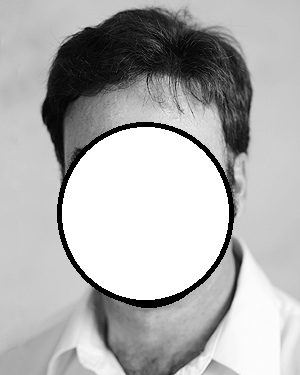
\includegraphics[width=1in,height=1.25in,clip,keepaspectratio]{author1.png}}]{First A. Author} received the B.S. and M.S. degrees in aerospace engineering from
the University of Virginia, Charlottesville, in 2001 and the Ph.D. degree in
mechanical engineering from Drexel University, Philadelphia, PA, in 2008.

From 2001 to 2004, he was a Research Assistant with the Princeton Plasma
Physics Laboratory. Since 2009, he has been an Assistant Professor with the
Mechanical Engineering Department, Texas A{\&}M University, College Station.
He is the author of three books, more than 150 articles, and more than 70
inventions. His research interests include high-pressure and high-density
nonthermal plasma discharge processes and applications, microscale plasma
discharges, discharges in liquids, spectroscopic diagnostics, plasma
propulsion, and innovation plasma applications. He is an Associate Editor of
the journal \emph{Earth, Moon, Planets}, and holds two patents.

Dr. Author was a recipient of the International Association of Geomagnetism
and Aeronomy Young Scientist Award for Excellence in 2008, and the IEEE
Electromagnetic Compatibility Society Best Symposium Paper Award in 2011.
\end{IEEEbiography}


\begin{IEEEbiography}[{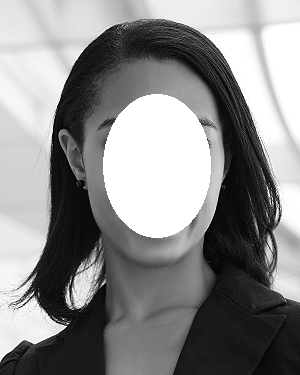
\includegraphics[width=1in,height=1.25in,clip,keepaspectratio]{author2.png}}]{Second B. Author} (M'76--SM'81--F'87) and all authors may include
biographies. Biographies are often not included in conference-related
papers. This author became a Member (M) of IEEE in 1976, a Senior
Member (SM) in 1981, and a Fellow (F) in 1987. The first paragraph may
contain a place and/or date of birth (list place, then date). Next,
the author's educational background is listed. The degrees should be
listed with type of degree in what field, which institution, city,
state, and country, and year the degree was earned. The author's major
field of study should be lower-cased.

The second paragraph uses the pronoun of the person (he or she) and not the
author's last name. It lists military and work experience, including summer
and fellowship jobs. Job titles are capitalized. The current job must have a
location; previous positions may be listed
without one. Information concerning previous publications may be included.
Try not to list more than three books or published articles. The format for
listing publishers of a book within the biography is: title of book
(publisher name, year) similar to a reference. Current and previous research
interests end the paragraph.

The third paragraph begins with the author's
title and last name (e.g., Dr.\ Smith, Prof.\ Jones, Mr.\ Kajor, Ms.\ Hunter).
List any memberships in professional societies other than the IEEE. Finally,
list any awards and work for IEEE committees and publications. If a
photograph is provided, it should be of good quality, and
professional-looking. Following are two examples of an author's biography.
\end{IEEEbiography}



\begin{IEEEbiography}[{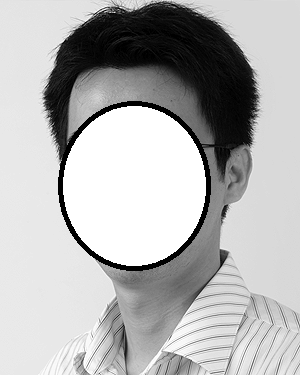
\includegraphics[width=1in,height=1.25in,clip,keepaspectratio]{author3.png}}]{Third C. Author, Jr.} (M'87) received the B.S. degree in mechanical
engineering from National Chung Cheng University, Chiayi, Taiwan, in 2004
and the M.S. degree in mechanical engineering from National Tsing Hua
University, Hsinchu, Taiwan, in 2006. He is currently pursuing the Ph.D.
degree in mechanical engineering at Texas A{\&}M University, College
Station, TX, USA.

From 2008 to 2009, he was a Research Assistant with the Institute of
Physics, Academia Sinica, Tapei, Taiwan. His research interest includes the
development of surface processing and biological/medical treatment
techniques using nonthermal atmospheric pressure plasmas, fundamental study
of plasma sources, and fabrication of micro- or nanostructured surfaces.

Mr. Author's awards and honors include the Frew Fellowship (Australian
Academy of Science), the I. I. Rabi Prize (APS), the European Frequency and
Time Forum Award, the Carl Zeiss Research Award, the William F. Meggers
Award and the Adolph Lomb Medal (OSA).
\end{IEEEbiography}

\EOD

\end{document}
